
%% bare_conf.tex
%% V1.4b
%% 2015/08/26
%% by Michael Shell
%% See:
%% http://www.michaelshell.org/
%% for current contact information.
%%
%% This is a skeleton file demonstrating the use of IEEEtran.cls
%% (requires IEEEtran.cls version 1.8b or later) with an IEEE
%% conference paper.
%%
%% Support sites:
%% http://www.michaelshell.org/tex/ieeetran/
%% http://www.ctan.org/pkg/ieeetran
%% and
%% http://www.ieee.org/

%%*************************************************************************
%% Legal Notice:
%% This code is offered as-is without any warranty either expressed or
%% implied; without even the implied warranty of MERCHANTABILITY or
	%% FITNESS FOR A PARTICULAR PURPOSE! 
%% User assumes all risk.
%% In no event shall the IEEE or any contributor to this code be liable for
%% any damages or losses, including, but not limited to, incidental,
%% consequential, or any other damages, resulting from the use or misuse
%% of any information contained here.
%%
%% All comments are the opinions of their respective authors and are not
%% necessarily endorsed by the IEEE.
%%
%% This work is distributed under the LaTeX Project Public License (LPPL)
%% ( http://www.latex-project.org/ ) version 1.3, and may be freely used,
%% distributed and modified. A copy of the LPPL, version 1.3, is included
%% in the base LaTeX documentation of all distributions of LaTeX released
%% 2003/12/01 or later.
%% Retain all contribution notices and credits.
%% ** Modified files should be clearly indicated as such, including  **
%% ** renaming them and changing author support contact information. **
%%*************************************************************************


% *** Authors should verify (and, if needed, correct) their LaTeX system  ***
% *** with the testflow diagnostic prior to trusting their LaTeX platform ***
% *** with production work. The IEEE's font choices and paper sizes can   ***
% *** trigger bugs that do not appear when using other class files.       ***                          ***
% The testflow support page is at:
% http://www.michaelshell.org/tex/testflow/



\documentclass[conference]{IEEEtran}
% Some Computer Society conferences also require the compsoc mode option,
% but others use the standard conference format.
%
% If IEEEtran.cls has not been installed into the LaTeX system files,
% manually specify the path to it like:
% \documentclass[conference]{../sty/IEEEtran}


% correct bad hyphenation here
\hyphenation{op-tical net-works semi-conduc-tor}


\usepackage{graphicx} % Required for the inclusion of images

\begin{document}
%
% paper title
% Titles are generally capitalized except for words such as a, an, and, as,
% at, but, by, for, in, nor, of, on, or, the, to and up, which are usually
% not capitalized unless they are the first or last word of the title.
% Linebreaks \\ can be used within to get better formatting as desired.
% Do not put math or special symbols in the title.
\title{Literature Survey of SHA-256 Hardware implementations for ECSE 682 project}


% author names and affiliations
% use a multiple column layout for up to three different
% affiliations
\author{\IEEEauthorblockN{Shabbir Hussain}
\IEEEauthorblockA{Dept. of Computer Engieering, 
McGill University\\
Montreal, Quebec\\
Email: shabbir.hussain@mail.mcgill.ca}
}

% make the title area
\maketitle

% As a general rule, do not put math, special symbols or citations
% in the abstract
\begin{abstract}
SHA-256 is a cryptographic one way hashing algorithm used to verify the authenticity of files and messages. It is a NIST standard used in many protocols such as SSH, PGP, IPSec and HMAC. This project compares a software implementation, versus a hardware implementation by a high level synthesis tool versus a fully hardware design implementation. The results show that in the hardware design implementation comes out ahead in terms of performance and area on a Cyclone V fpga. 
\end{abstract}

\IEEEpeerreviewmaketitle

\section{Introduction} \label{introduction}
Cryptography is often known as a practice to send secret messages. While encrypting and decrypting messages are an important part of keeping secrets, so too is the method of verifying that message content is unaltered from sender to receiver. One of the methods employed to make sure that a message remains unmodified in transit is called a Message Authentication Code (MAC). These codes are computed based on the message contents and a shared secret key between sender and receiver. A MAC provides message integrity because an imposter can not feasibly create a false message and MAC pair or modify the contents of an existing message that will trick the receiver into believing that the messages were authored by the true sender \cite{schneier}. This is because the generation and verification of a MAC involves using a cryptographically secure hash function such as the SHA-256 algorithm. The SHA-256 algorithm is a NIST standard that is part of a family hash functions called the SHA2 family. These functions take as input an arbitrary length string of bits and compute fixed length string of bits called the Digest Message (DM). These functions are one way functions with a low chance of collisions. Changing 1 bit of the input dramatically changes the output making it very difficult to guess the input based on the output. This property is what gives it its relevance in the field of cryptography. The only way to compute the input a DM is to guess and as of writing this paper there no known attacks on the SHA-256 to speed up this process. Given a 256 bit DM it would take a modern computer several years to find the corresponding input. This is because cryptographic functions are slow in general.\\ Computing a MAC for every message adds a performance and power penalty. IPSec’s performance bottleneck is the HMAC mechanism which
is responsible for authenticating the transmitted data \cite{michail}. VLSI is literature is rich in solutions that offload the has computation to hardware to quickly compute hashes with a low area foot print. \\
This paper presents three implementations of the SHA-256 algorithm. The first approach is a fully software implementation run on a 12 core,Intel(R) Xeon(R) @ 2.50GHz computer located at legup.ece.mcgill.ca. The second approach sinthesises several implementations using the Legup High Level Synthesis (HLS) tool. The third approach implements the algorithm directly into an FPGA. This project compares all thee approaches on the metric of throughput measured in bits per second (bps). Also it compares the last two approaches in on the metric of area on a an fpga in terms of logic elements used. The Objective of this project is two fold. First and foremost, it is to learn about the advantages and disadvantage of using an HLS tool as well as learning application specific VLSI design techniques. Second, it is to measure the performance gains over an HLS tool when designing a hardware implementation of a specific algorithm.

\section{SHA-256 algorithm} \label{sha256}
The SHA-256 algorithm takes in a bit string of a maximum size of $2^{64}$ bits and outputs a 256-bit output called the Digest Message (DM) \cite{nist}. The SHA-256 algorithm can be divided into three steps.
\begin{enumerate}
  \item Padding
  \item Data Initialisation
  \item Round Hashing
\end{enumerate}

During the Padding step, the input message is subdivided into 512 bit blocks. The last block is padded to a multiple of 512 bits. At the end of the contents of the last block a 1 bit is placed followed by zeroes. The last 64 bits of that block are used to store the message length. Figure \ref{fig:pad} show an example of a padded input. 

The next step is the data Initialisation. In this step many variables are initialized to values specified by the National Institute of Standards and Technology \cite{nist}. The DM takes its initial value, the constants take their values, and the message block is loaded into a vector called the message schedule. The initialization of the message schedule is show in figure \ref{fig:messageSchedule}. 

The round hashing step happens once for every message block. During this round, the initial digest message is broken into 8 32-bit components and manipulated by a set of rotations and combinational logic 64 times in an inner loop. This inner loop can be seen in Figure \ref{fig:innerloop}. The functions in the inner loop and data initialization (sigma, MAJ, etc.) are combinational logic functions defined by NIST \cite{nist}. Finally, the after all the rounds are completed the digest message is recombined into a 512-bit format which is the result of the hash.

\begin{figure}[!t]
\centering
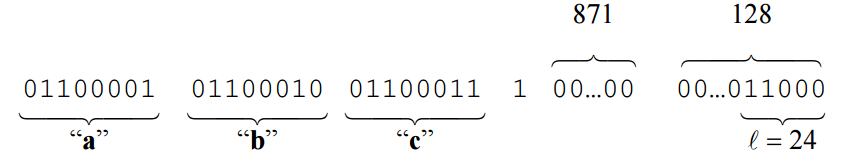
\includegraphics[width=2.5in]{padding}
\caption{An example of the SHA-256 padding}
\label{fig:pad}
\end{figure}


\begin{figure}[!t]
\centering
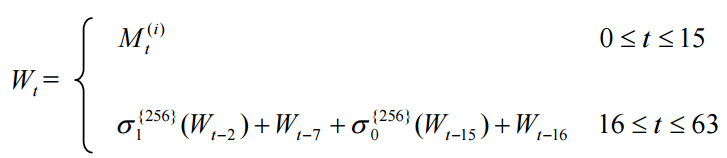
\includegraphics[width=2.5in]{messageSchedule}
\caption{The generation of the Message Schedule vector (W) based on the input Message (M)}
\label{fig:messageSchedule}
\end{figure}

\begin{figure}[!t]
\centering
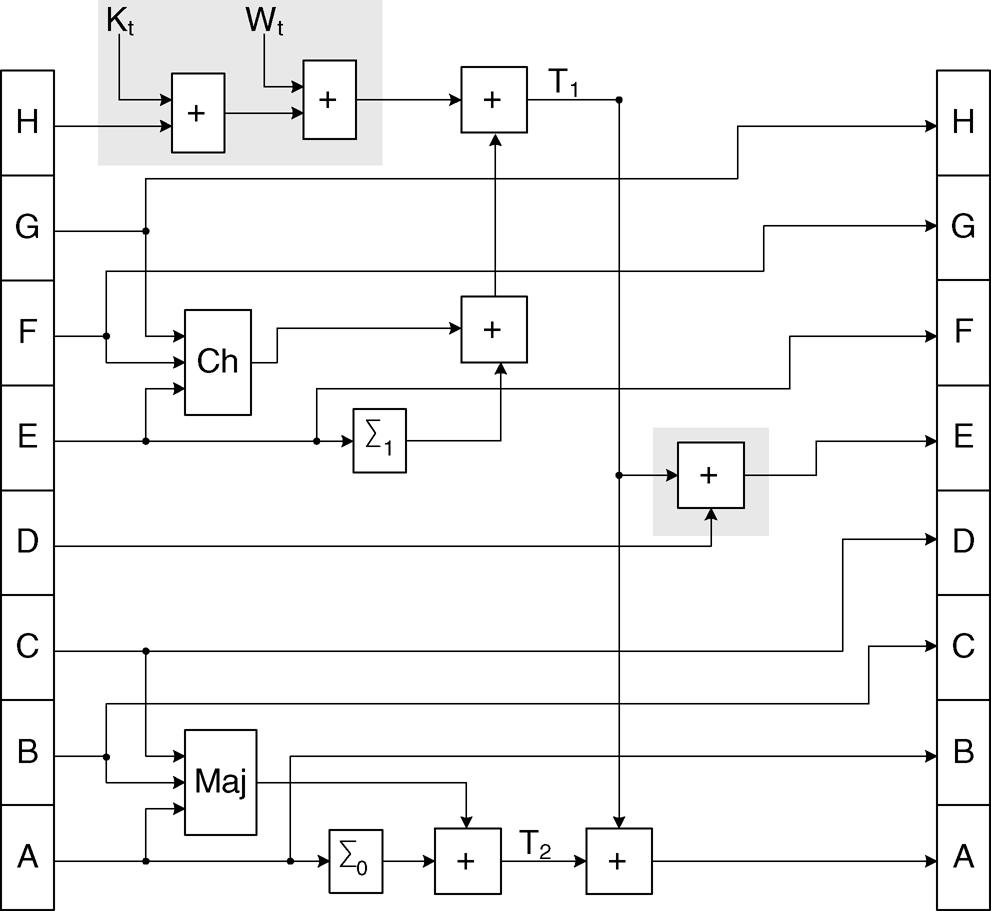
\includegraphics[width=2.5in]{sha2round}
\caption{One round of the inner loop of the SHA-256 algorithm}
\label{fig:innerloop}
\end{figure}


\section{Software} \label{Software}
The software implementation of the algorithm was written in C. Many C implementations exists already, such as the implementation in the OpenSSL library. However, a redesign from the ground up was the chosen route for two reasons. Firstly, it was for the educational benefit of the author. Secondly, this implementation needs to have the no amount of dependencies to libraries that are not compatible with the Legup HLS tool. This is so that the software implementation can serve as a building block for the legup HLS tool. 

The C implementation followed the algorithm as described in \cite{nist}. In order to verify correctness, several inputs were compared to existing implementations. Some of the test cases are described in table \ref{tab:tests}. The actual inputs are too large to display in this format and are omitted. These cases were chosen to test as many blocks of the code. For example, the no input case would test the inner loop of the program. If all operations are correct then the initial hash should be changed to "e3b0c44298fc1c149afbf4c8996fb92427ae41e4649b934ca495\\991b7852b855". An incorrect output could isolate an error at the inner loop block. 

\begin{table}
\begin{center}
	\caption{Test cases to verify correctness of SHA-256 algorithm}
    \begin{tabular}{| l | l |}
    \hline
    \label{tab:tests}
    Equivalence case	 & Passing \\ \hline\hline
	No Input & True \\ \hline
	One block & True\\ \hline
	Two blocks & True \\ \hline
	All letters & True \\ \hline
	256 letters & True \\  \hline
    \hline 
    \end{tabular} 
\end{center}  
\end{table}

Once the code was completed it was measured for performance using a Gprof \cite{gprof}. Gprof is a profiling tool for C code used to measure execution time. Grof was able to accurately measure the execution time of the program to 4us. The program processed 512 bits. Using the formula $Throughput = bits/time$ we can calculate thoughput as $(512 bits)/(4us) = 128 Mbps$. These measurements were made on a relatively fast 12 core, Intel(R) Xeon(R) @ 2.50GHz computer. This computer is located at legeup.ece.mcgill.ca. This speed is impressive considering it is a fully sequential software implementation and reaches a throughput in the same order of magnitude to that of the implementation of \cite{sklav} which had a throughput of 291 Mbps.

A tool call callgrind \cite{callgrind} was also used to profile the code. Callgrind outputs a nice visual representation of the execution time of each method of the program. This feature is useful for identifying hot spots in the program. Figure \ref{fig:profile} shows the visual representation of the program execution. It is clear that the two most time consuming parts of the application are the padding (brown) and the round steps (red). This is expected because round steps are very sequential in the software implementation. We will use this information to speed up the hardware implementation in section \ref{Hardware}. 

\begin{figure}[!t]
\centering
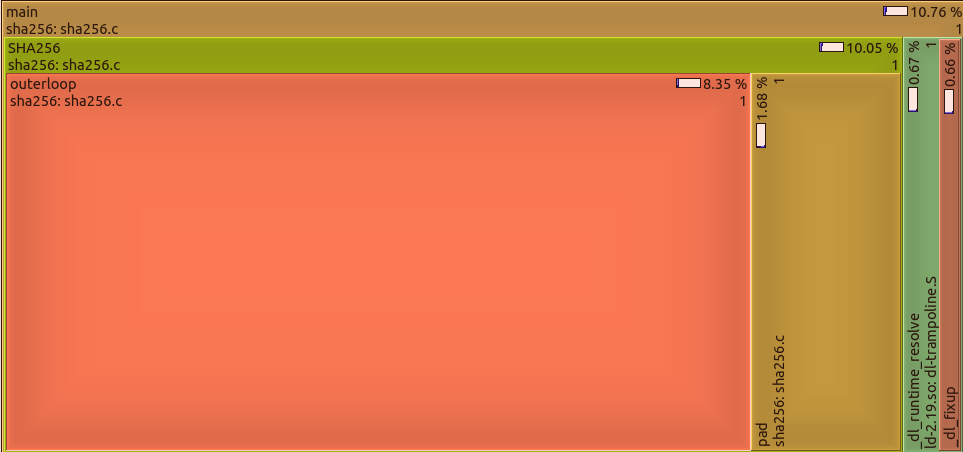
\includegraphics[width=2.5in]{executionTime}
\caption{Callgrind view of the program execution}
\label{fig:profile}
\end{figure}


\section{Legup} \label{Legup}
Legup is a HLS tool which is able to take C code and compile it down to synthesisable verilog. The code from section \ref{Software} was reused in this section as the input to the Legup HLS tool. The setup requires the code to be located at legup.ece.mcgill.ca, a specialised make file and a specialised tcl file. The make file specifies the program, the location of the tcl and the location of other make targets. In this project the targets of the default Legup program were used by including the contents of Legup4.0/examples/Makefile.common. The tcl file specifies the FPGA board as well as sections of the code to parallelize. The hardware target for this design was the Cyclone IV DE2 board and also the Cyclone V GX board.  

Several different configurations were tested to learn how a well an HLS tool can synthesize a given algorithm. The three legup designs are the full software implementation, the full hardware implementation and the openmp parallelized implementation. Unfortunately, the hybrid flow and loop pipelining flow were incompatible with this project. A full summary of all the implementations can be seen in table \ref{tab:Legup}.

\subsection{Software flow implementation}
Legup provides a software flow implementation. This flow compiles the C code for a MIPS processor. The MIPS processor runs at 50Mhz. When compiled with the make target $make  sw$ the tigerMIPS processor is copied to working directory. Then to simulate the code the target $make swsim$ was run. The resulting simulation ran in 4034 cycles. To calculate the throughput we can use $Throughput = bits *ClockRate / (cycles)$. In this case we obtain $512 bits * 50Mhz/4034 cycles = 6.32Mbps$. Which is very poor compared to previous software implementation. However, it is important to note that this processor is much slower.

\subsection{Hardware flow implementation}
Legup's default flow is the hardware flow. This flow takes the C code and compiles it down to synthesizable verilog, which we can then synthesize for our board. This whole flow is done with three targets $make hw$, $make p$, $make f$. The first target compiles the C code down to verilog, the second target creates a quartus project with the Cyclone IV DE-2 board as a target, the third target does does a full compilation for the target board. After this compilation process we can view the compilation reports to obtain the maximum clock frequency and the hardware utilization. We also run the target $make v$ to simulate the program in modelsim in order to obtain the number of clock cycles required to Hash 512 bits. From the reports  we obtain an Fmax of 82.6Mhz. From the simulation we obtain a run time of 1677 cycles. We can then compute the  Throughput to be $512*82.6/1677= 25.21Mbps$. 

\subsection{OpenMP parallelization flow}
This flow work the same as the previous, however, we change two pieces of the source. First in the source we add open mp pragmas to select pieces of the code where parallelism would improve performance. We parallelize the data initialization and the innerloop. Figure \ref{fig:datainitparallel} and figure \ref{fig:innerloopparallel} show the open mp pragmas. Second, we add to a parameter to the tcl file to enable open mp parallelization. From this flow we obtained an Fmax of 84.87 Mhz and a simulation of 2237 cycles which resulted in a throughput of $512*84.87/2237=19.42Mbps$. Although it has a faster clock rate, it required more execution cycles to complete. This is most likely due to the overhead of using a large number of threads.


\begin{figure}[!t]
\centering
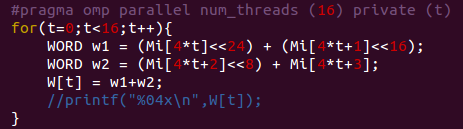
\includegraphics[width=2.5in]{datainitparallel}
\caption{Parallelizing the Data initialization}
\label{fig:datainitparallel}
\end{figure}

\begin{figure}[!t]
\centering
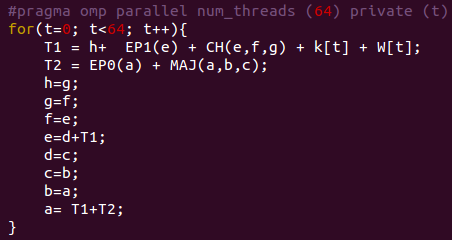
\includegraphics[width=2.5in]{innerLoopParallel}
\caption{Parallelizing the inner loop}
\label{fig:innerloopparallel}
\end{figure}


\subsection{Hardware flow on Cyclone V}
In order to verify the change in performance and area on a different generation of FPGA, the parallel hardware flow was recompiled for the Cyclone V. To do so, the tcl file parameter for hardware target was change to the Cyclone V. From this flow we obtained an Fmax of 130 Mhz and a simulation of 2237 cycles which resulted in a throughput of $512*130/2237=29.75Mbps$. This implementation also used less area. This is shows that the synthesis from verilog to FPGA also impacts performance and area. It demonstrates that one can dramatically improve an algorithm by improving the underlying hardware.

\subsection{Legup discussion}
The Legup implementations were each incrementally better than other but not better than the pure software implementation from section \ref{Software}. To investigate why, we used the RTL viewer tool from quartus to see inside the model generated by Legup. We can see  in figure \ref{fig:sha256module} that it implements each function as a module. Looking further into a module was not fruitful since the RTL view gets messy as seen in figure \ref{fig:rtlmess}. Only when looking into the generated verilog can we see that legup uses predefined functional units which bloat the system. For example, the verilog design has a dual port RAM for every array in the C code. This adds  to the area since the C code does not need to access all the arrays in parallel. Moreover, it requires many cycles due to the numerous memory accesses. In the next section, we take advantage of this  knowledge to create an improved hardware design.


\begin{figure}[!t]
\centering
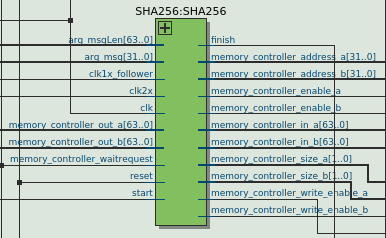
\includegraphics[width=2.5in]{sha256module}
\caption{The RTL view of the SHA-256 module}
\label{fig:sha256module}
\end{figure}

\begin{figure}[!t]
\centering
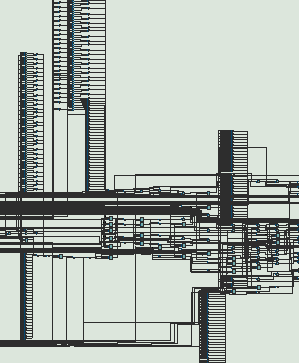
\includegraphics[width=2.5in]{rtlmess}
\caption{The RTL view inside the SHA-256 module}
\label{fig:rtlmess}
\end{figure}

	

\begin{table}
\begin{center}
	\caption{Test cases to verify correctness of SHA-256 algorithm}
    \begin{tabular}{| l | l | l |}
    \hline
    \label{tab:Legup}
    Flow 	 & Throughput & Area \\ \hline\hline
	Software & 6.32 Mbps & -  \\ \hline
	Hardware & 25.21 Mbps & 6133 \\ \hline
	Hardware Parallel Cyclone IV & 19.42 Mbps &  5959 \\ \hline
	Hardware Parallel Cyclone V & 29.75 Mbps &  2294 \\ \hline
	
    \hline 
    \end{tabular} 
\end{center}  
\end{table}

\section{Hardware} \label{Hardware}
The hardware design of the algorithm was implemented on a Cyclone V board using verilog. This design implemented the algorithm directly from specification \cite{nist} to verilog. A high level design diagram is seen in figure \ref{fig:highleveldgm}. The design shows a control block controlling two functional unit that haves access to a RAM. This ram is where the inputs are stored and is also where the outputs will be stored. The control logic controls the sequence of computation such that the data is first padded and then processed by the round computation unit. 
The RAM block holds space for the initial data block (512 bits) and the final output digest (256 bits). The RAM is a synchronized single port RAM which reads or writes 1 byte at a time. This makes it easy to read and write ascii strings. 

The padder unit takes in as input the length of the input from the control block. Using that information, it writes the pad to RAM assuming that data in the RAM starts at address 0. It then signals to the control block that it is done.

When the padder has completed its task, the control block signals the round computation unit to begin. The round computation computes some of the data initialization during when the reset signal is high. It then initializes the scheduling vector (W) by reading elements from the memory. Unlike the Legup implementation, the scheduling vector (W) is stored locally within registers. Next it runs through the inner loop computations and lastly it writes the computed hash values to RAM. The round computation unit also has a ROM which stores the constants of the SHA-256 algorithm. This idea was adopted from \cite{sklav} and reduces the need to access RAM memory thus speeding up the computation.

This design went through an iterative design process where some techniques from the literature \cite{michail} \cite{ceshar} were attempted in order to increase the throughput. The rest of this section will go through some of the design choices in each iterative step.

\begin{figure}[!t]
\centering
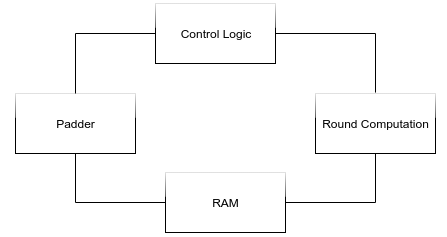
\includegraphics[width=2.5in]{highleveldgm}
\caption{Parallelizing the inner loop}
\label{fig:highleveldgm}
\end{figure}

\subsection{Loop unrolling}
The first design choice was to unroll the inner loop. The design from \cite{michail} unrolled the innerloop twice. Unrolling a loop lengthens the critical path, however, if the critical path is not located in the loop then we can unroll the loop and see an increase in throughput because we are doing more work in one clock cycle. For our first design we fully unrolled the inner loop (64 times unrolled). A fully unrolled loop finished in very few clock cycles but also had a very slow clock. The resulting throughput was a meagre $11.63 Mbps$ which can be seen in table \ref{tab:hardware}. The second design had the loop unrolled twice and saw a jump in throughput to $215 Mbps$. The third design had no loop unrolling and had a throughput of $248 Mbps$. From these results it is clear that the critical path is shorter than two unrolled loops and therefore no unrolling is best. 


\subsection{Pipelining}
Pipelining can also reduce the critical path. The design in \cite{ceshar} uses pipeining to speed up the compuation of the scheduling vector. In our design we recreate this block as seen in figure \ref{fig:fifosched}. We create a Fifo which stores values of the scheduling vector. We also create three extra registers which contain partial computations of the values of the scheduling vector. Figure \ref{fig:wschedpip} shows how the scheduling vector computation can be broken down into three additions that occur at three different time steps. The result from this section can also be seen in table \ref{tab:hardware}. From this implementation we achieved a throughput of 298 Mbps. That result is more than twice as fast as the software only implementation, ten times faster than the best legup implementation and faster than the implementation in \cite{sklav}. From the results we can see that there is no improvements in the number of cycles required for the computation but there is a major gain in the clock frequency. This indicates that the scheduling vector calculation was part of the critical path and pipelining reduced it.


\begin{figure}[!t]
\centering
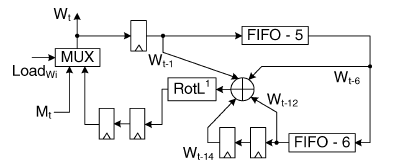
\includegraphics[width=2.5in]{fifosched}
\caption{Fifo based data initialization block from \cite{ceshar} }
\label{fig:fifosched}
\end{figure}


\begin{figure}[!t]
\centering
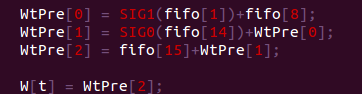
\includegraphics[width=2.5in]{wshcedpip}
\caption{Breakdown of the scheduling vector additions}
\label{fig:wschedpip}
\end{figure}

\subsection{discussion}
In this section we implemented the SHA-256 algorithm directly from specification to verilog. Then applied various techniques from the literature to speed up our results. 

One attribute all these designs have is that they consistently use less area than the Legup synthesis. This can be attributed to the lack of bloat-ware. For example, this design uses exactly enough RAM for one block of input and one hash value. Reducing area footprint can be a potential for future research for the Legup HLS.

 The lessons learned are that loop unrolling is inefficient if it increases critical path. Also pipelining will reduce critical path but not the number of cycles required to compute an answer. To further improve this design we can modify the RAM. A RAM that reads and writes 8 bits at a time also places a bottleneck since the rest of the algorithm uses 32 bit chunks of data. We can surely improve the number of clock cycles required to process the data if we were able to load in 32 bits at a time. Moreover, we can try to compute several SHA hashes at once as in \cite{michail}, since our padder unit is left idle when the round computation unit is active.



\begin{table}
\begin{center}
	\caption{Test cases to verify correctness of SHA-256 algorithm}
    \begin{tabular}{| l | l | l | l | l |}
    \hline
    \label{tab:hardware}
    Technique 	 & Cycles & Fmax & Throughput & Area \\ \hline\hline
	Fully unrolled loop & 158 & 3.59Mhz & 11.63 Mbps & 2054  \\ \hline
	Twice Unroolled loop & 191 & 80.55 Mhz & 215.92 Mbps & 944 \\ \hline
	No Unrolling	 & 223 &  108.15 & 248.3 Mbps &  912 \\ \hline
	Pipelining & 223 & 130.19 Mhz & 298.91 Mbps &  631 \\ \hline
	
    \hline 
    \end{tabular} 
\end{center}  
\end{table}


\section{Conclusion} \label{Conclusion}
This project explored three different implementations of the SHA-256 algorithm in order to learn about HLS tools and application specific hardware design. First, a software only design was implemented and profiled as a benchmark to compare against. Second, using Legup, a HLS tool, a second design was synthesized. This design didn't fair very well against the software only design. It demonstrates that simply putting an algorithm onto hardware does not automatically speed it up. Lastly, a fully hardware design was implemented. This design had a higher throughput than the software design, all of the Legup designs and the design in \cite{sklav}. Since legup is a HLS tool which can synthesize any application code, the hardware design demonstrates that an application specific design tends to have better performance and area metrics than a HLS tool. 


% http://www.michaelshell.org/tex/ieeetran/bibtex/
\bibliographystyle{IEEEtran}
% argument is your BibTeX string definitions and bibliography database(s)
\bibliography{shabibl}


% that's all folks
\end{document}


